% Para compilar, use:
% pdflatex -shell-escape melissa_kthxbai.tex
%%%%%%%%%%%%%%%%%%%%%%%%%%%%%%%%%%%%%%%%%%%%%%%%%%%%%%%%%%%%%%%%%%%%%%%%%%%%%%%%%%%%%%%%%
% PREAMBULO
%%%%%%%%%%%%%%%%%%%%%%%%%%%%%%%%%%%%%%%%%%%%%%%%%%%%%%%%%%%%%%%%%%%%%%%%%%%%%%%%%%%%%%%%%
\documentclass{beamer}
% Temas do beamer
\usetheme{Boadilla}
%\usecolortheme{purple}
\usefonttheme[onlysmall]{structurebold}
\usenavigationsymbolstemplate{}
%\useoutertheme{smoothbars}
% This Charming Man palette from colorlovers.com
\definecolor{purple}{rgb}{0.5,0,0.5}
% Escolhendo as cores padrão do beamer
%\setbeamercolor{normal text}{fg=winterbland}
\setbeamercolor{structure}{fg=purple}
%\setbeamercolor{block title}{fg=lazereyes}
%\setbeamercolor{block body}{}
\setbeamercolor{alerted text}{fg=purple}
\setbeamercolor{frametitle}{fg=purple}
% % Customizações
% \setbeamertemplate{title page}
% {%
%    \vspace{2cm}
%    \begin{center}
%       \begin{minipage}{0.9\textwidth}
%          \begin{alertblock}{}
%             \vspace{0.5cm}
%             \begin{center}
%                \huge{\alert{\inserttitle}}
%             \end{center}
%             \vspace{0.5cm}
%          \end{alertblock}
%       \end{minipage}
%    \end{center}
%    \vspace{1cm}
%    \begin{center}
%       \large{\insertauthor}\\
%    \end{center}
%    \vspace{1cm}
%    \begin{flushright}
%       \small{\insertdate}
%    \end{flushright}
% }
% \setbeamertemplate{footline}
% {%
%    \flushright{\insertframenumber / \inserttotalframenumber}
%    \begin{beamercolorbox}[wd=.333333\paperwidth,ht=2.25ex,dp=1ex,right]{}
%    \end{beamercolorbox}
% }
% \pgfdeclarehorizontalshading[frametitle.bg,frametitle right.bg]{beamer@frametitleshade}{\paperheight}{%
%   color(0pt)=(frametitle.bg);
%   color(\paperwidth)=(frametitle right.bg)}
% \AtBeginDocument%
% {
%   \pgfdeclareverticalshading{beamer@topshade}{\paperwidth}{%
%     color(0pt)=(bg);
%     color(4pt)=(black!50!bg)}
%   \pgfdeclareverticalshading{beamer@bottomshade}{\paperwidth}{%
%      color(0pt)=(black!50!bg);
%      color(4pt)=(bg)}
% }
% \addtobeamertemplate{headline}
% {}
% {%
%   \vskip-0.2pt
%   \pgfuseshading{beamer@topshade}
%   \vskip-2pt
% }
% \addtobeamertemplate{footline}
% {}
% {%
%   \vskip-2pt
%   \pgfuseshading{beamer@bottomshade}
% }
\setbeamerfont{frametitle}{family=\bfseries}
\setbeamerfont{title}{family=\bfseries}
\AtBeginSection{\frame{\tableofcontents[currentsection,hideallsubsections]}}
%
% Pacotes adicionais
\usepackage[utf8]{inputenc} % Para permitir a exibição correta de acentos
\usepackage[portuguese]{babel} % Para exibir palavras-chave em português
\usepackage{txfonts} % Fontes bonitas :)
\usepackage{ctable}
\usepackage{colortbl}

% Variáveis da apresentação
\title{Software Livre na Matemática}
\author{Melissa Weber Mendonça}
\date{}
%%%%%%%%%%%%%%%%%%%%%%%%%%%%%%%%%%%%%%%%%%%%%%%%%%%%%%%%%%%%%%%%%%%%%%%%%%%%%%%%%%%%%%%%%
% FIM DO PREAMBULO
%%%%%%%%%%%%%%%%%%%%%%%%%%%%%%%%%%%%%%%%%%%%%%%%%%%%%%%%%%%%%%%%%%%%%%%%%%%%%%%%%%%%%%%%%

\begin{document}

{% Definindo frame de título.
\setbeamertemplate{footline}{} 
\setbeamertemplate{headline}{}
% \usebackgroundtemplate{\includegraphics[width=\paperwidth,height=\paperheight]{imagens/linus.jpg}}%
\begin{frame}%

   \titlepage%
   
\end{frame}%
 }

\begin{frame}
   \frametitle{O que é \emph{Software Livre}?}
   \begin{center}
     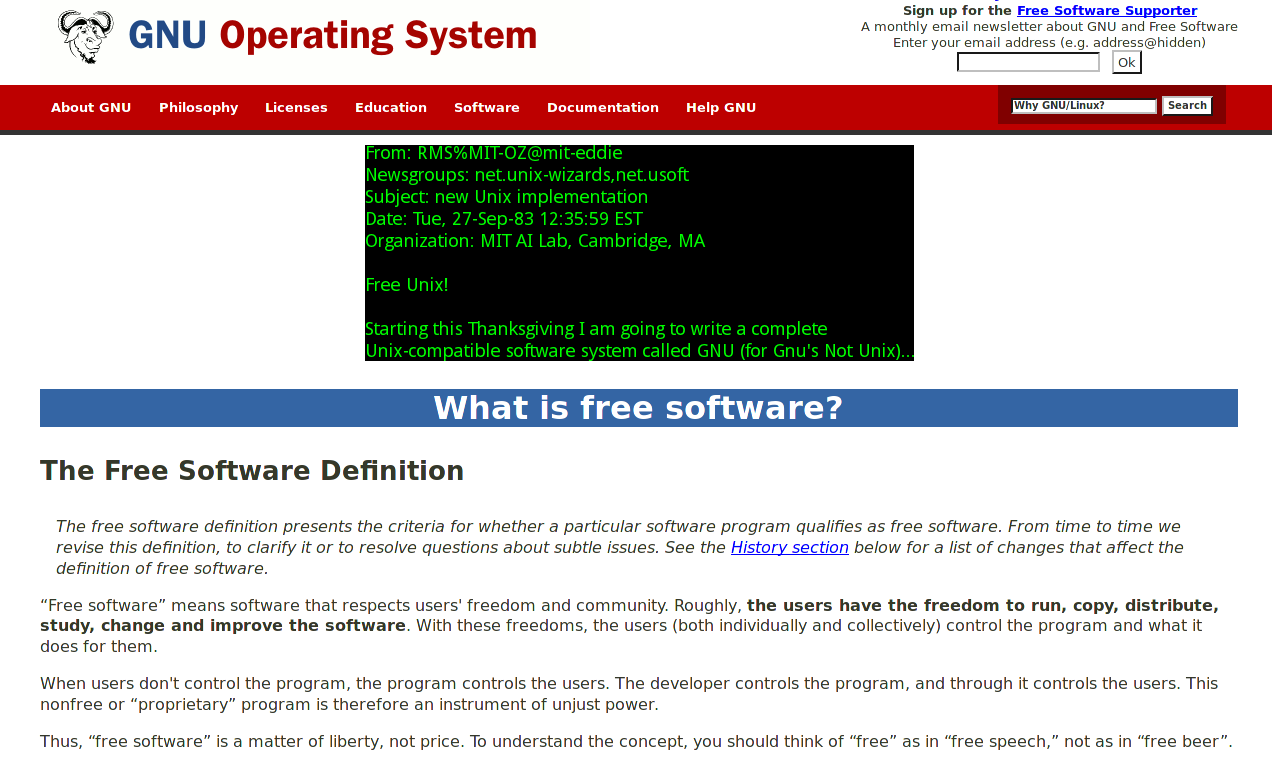
\includegraphics[width=\textwidth]{gnu_free.png}
   \end{center}
\end{frame}

\begin{frame}
   \frametitle{Richard Stallman e o Manifesto GNU}
   \begin{columns}
     \column{6cm}
     \begin{itemize}
       \item 1983: \emph{GNU's Not Unix}
       \item 1985: Free Software Foundation
     \end{itemize}
     \column{4.5cm}
     \begin{center}
       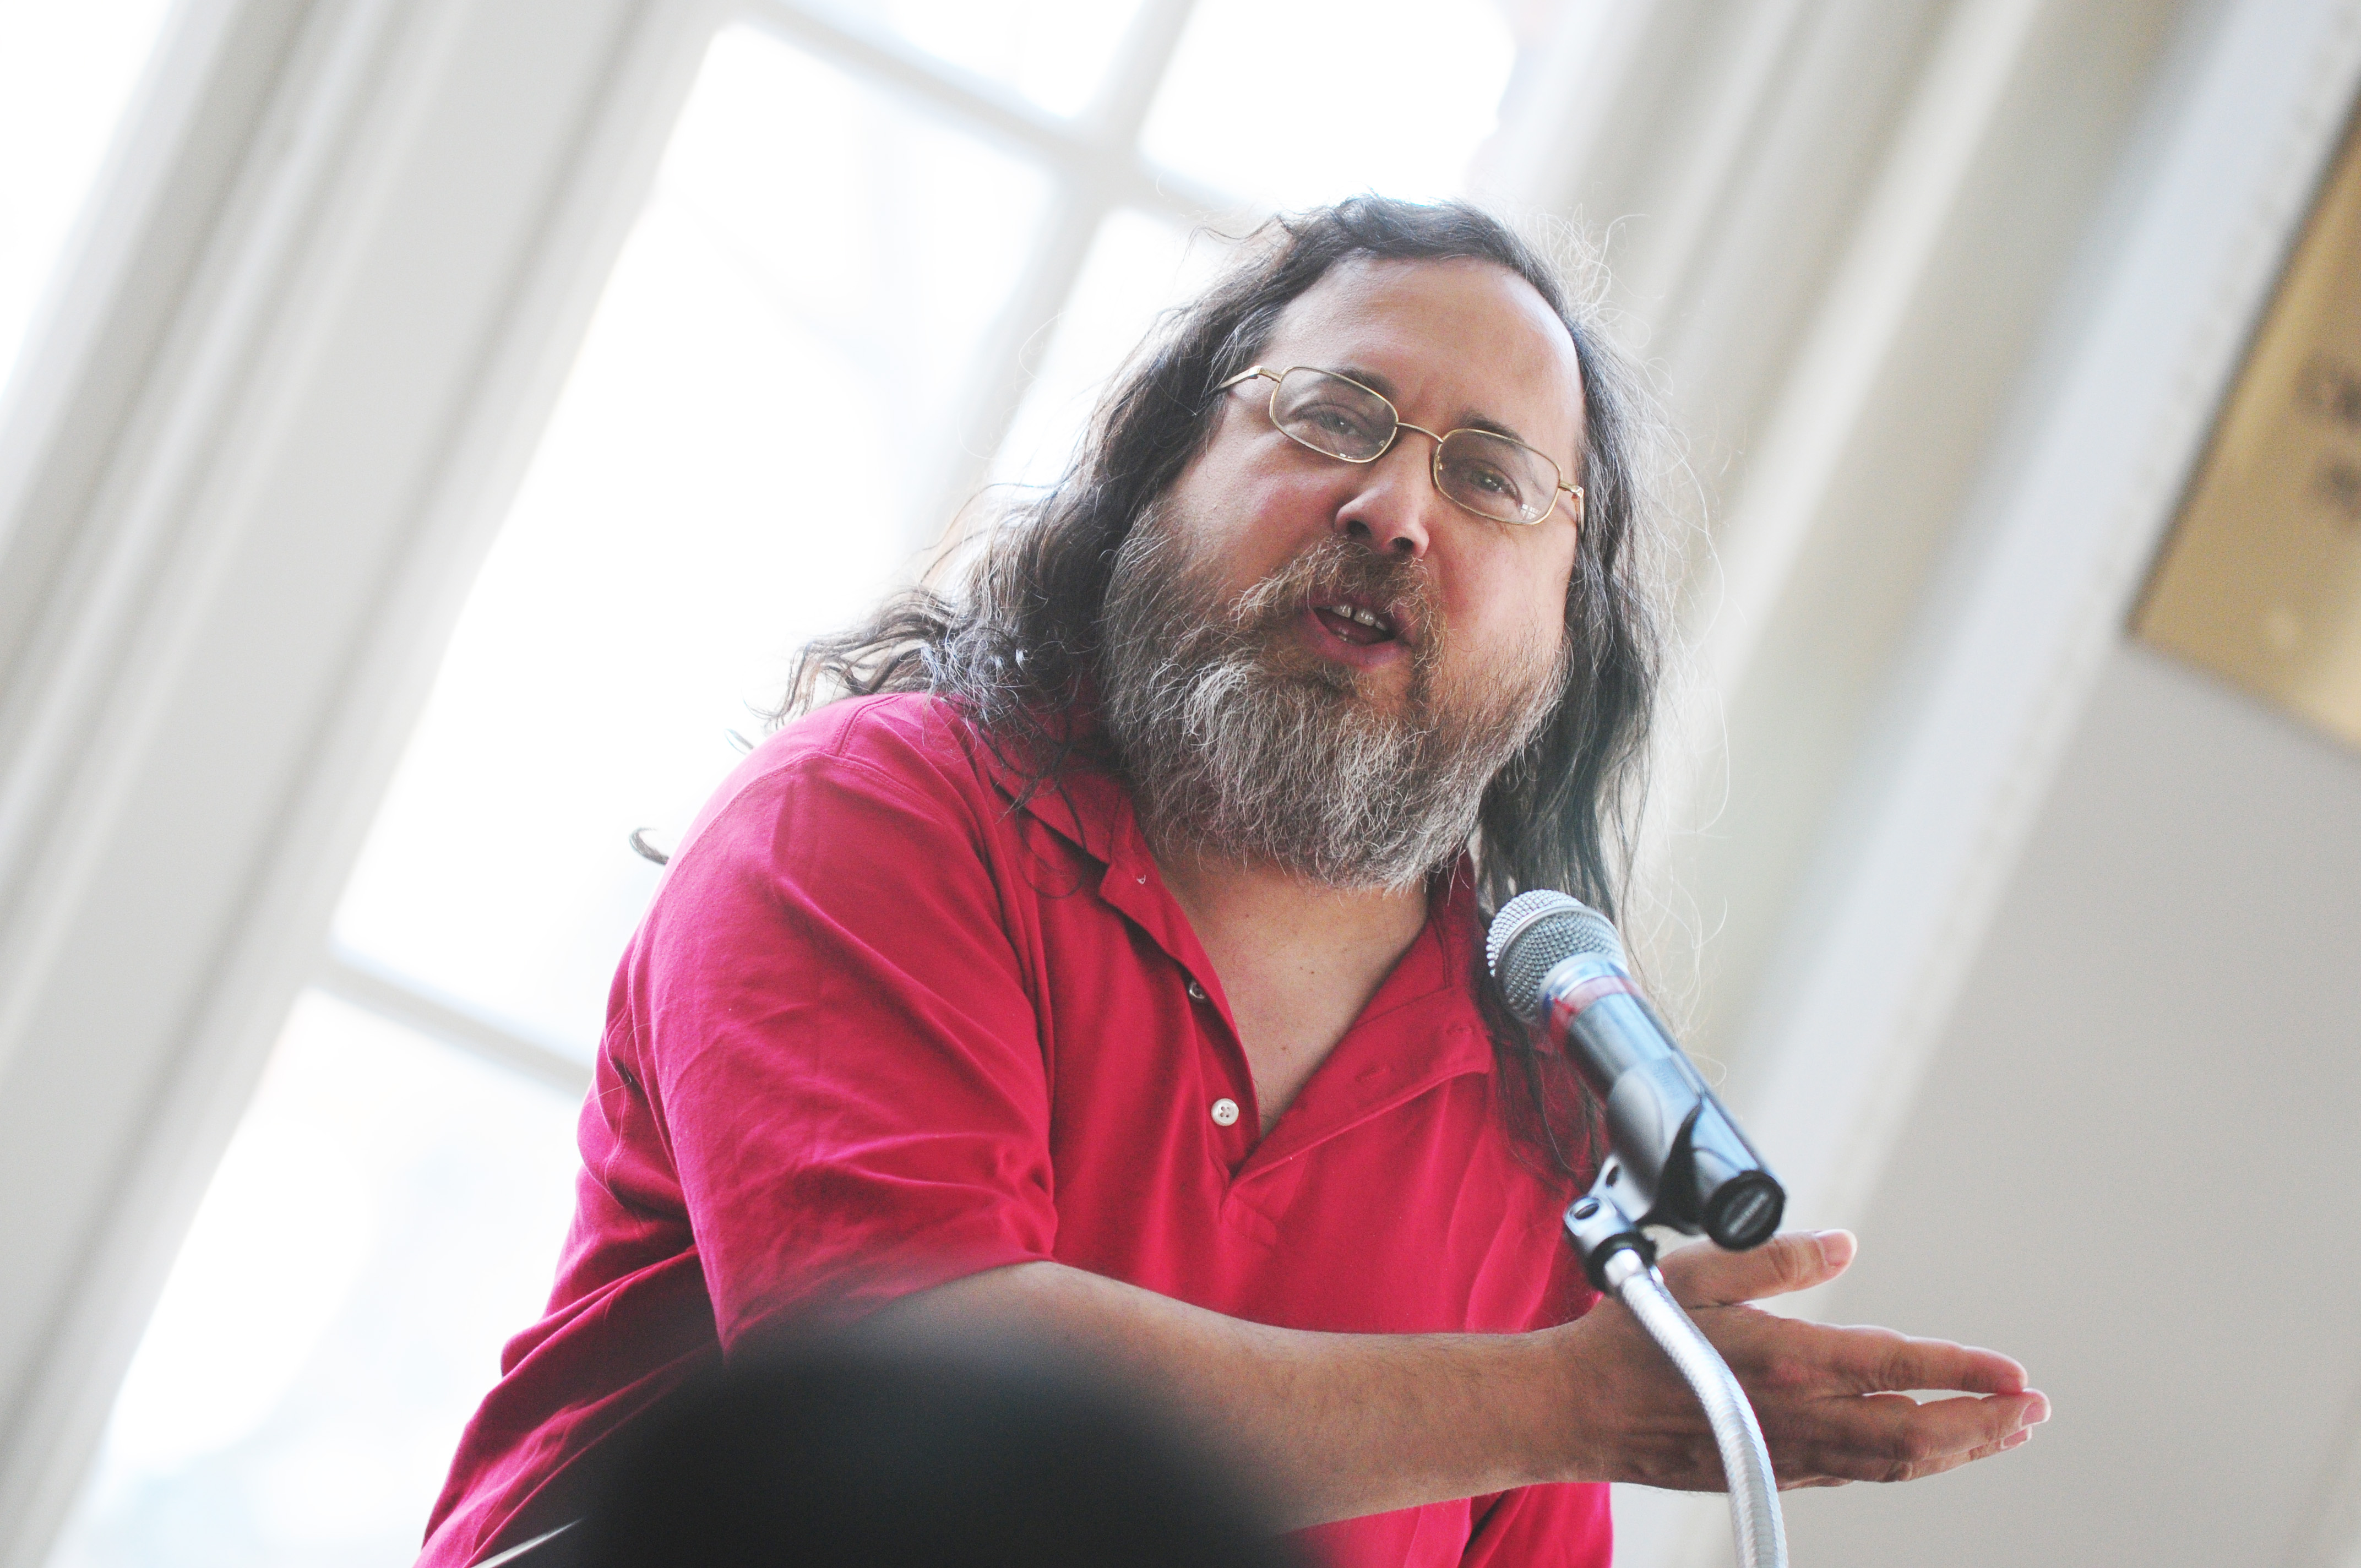
\includegraphics[width=4.5cm,trim=40mm 0mm 40mm 0mm,clip]{stallman.jpg}\\
       rms
     \end{center}
   \end{columns}
   \begin{center}
     ``The principal goal of GNU is to be free software. Even if GNU had no technical advantage over Unix, it would have a social advantage, allowing users to cooperate, and an ethical advantage, respecting the user's freedom.''
   \end{center}
\end{frame}

\begin{frame}
  \frametitle{As liberdades}
  \begin{block}{}
  \begin{description}[<+->]
  \item[Liberdade 0] O usuário deve poder executar o programa, para qualquer fim.
  \item[Liberdade 1] O usuário deve poder estudar como o programa funciona, e fazer modificações para que o resultado seja o que ele deseja. (código aberto)
  \item[Liberdade 2] O usuário deve poder redistribuir cópias do programa para sua comunidade.
  \item[Liberdade 3] O usuário deve poder redistribuir suas cópias modificadas.
  \end{description}
  \end{block}
\end{frame}

\begin{frame}
   \frametitle{\emph{``Free as in beer''} vs. \emph{``Free as in speech''}}
   \begin{center}
     \begin{minipage}{0.8\textwidth}
       \begin{block}{}
         \begin{center}
           Software Livre não é necessariamente grátis!
         \end{center}
       \end{block}
     \end{minipage}
   \end{center}
\end{frame}

\begin{frame}
   \frametitle{Licenças Livres}
   \begin{itemize}
   \item Copyleft é uma subversão da lei de copyright: ao invés de restringir um programa, exige que ele seja livre.
   \item Impede que alguém faça uma modificação a um software livre e aplique uma licença proprietária.
   \item Contagiosa: impede que se combine software livre e proprietário com uma licença proprietária
   \end{itemize}
   \begin{columns}
     \column{4cm}
     \begin{center}
       
\includegraphics[width=3cm]{copyleft.png}
     \end{center}
     \column{7cm}
     \begin{center}
       
\includegraphics[width=5cm]{GPLv3_Logo.png}
     \end{center}
 \end{columns}
\end{frame}

\begin{frame}
  \frametitle{Licenças Livres}
  \begin{itemize}
  \item Apache
  \item BSD
  \item LaTeX Project Public License
  \item Microsoft Public License (Ms-PL)
  \item Mozilla Public License (MPL)
  \item Domínio Público
  %\item The GPL-PA (“Licença Pública Geral para Administração Pública”) não é free
  \end{itemize}
\end{frame}

\begin{frame}
  \frametitle{Creative Commons}
  Para trabalho artístico ou criativo (fotos, imagens, música, produção literária...)
  \begin{itemize}
  \item CC BY: Atribuição; trabalho pode ser modificado e a modificação pode ser usada comercialmente;
  \item CC BY-SA: CC BY + deve manter a mesma licença do original (copyleft);
  \item CC BY-ND: Atribuição; trabalho pode ser comercializado e redistribuído, mas sem modificações;
  \item CC BY-NC: Atribuição; trabalho pode ser modificado e redistribuído, não comercialmente.
  \item CC BY-NC-SA
  \item CC BY-NC-ND
  \end{itemize}
\end{frame}

\begin{frame}
   \frametitle{Open Source vs. Free Software}
   \begin{columns}
     \column{8cm}
     \begin{center}
     Todo software livre é \emph{open source} (código aberto) mas nem todo código aberto é software livre!\\
     \vskip2cm
     
\includegraphics[width=2cm]{osi-logo.png}
   \end{center}
   \column{3cm}
   \begin{center}
     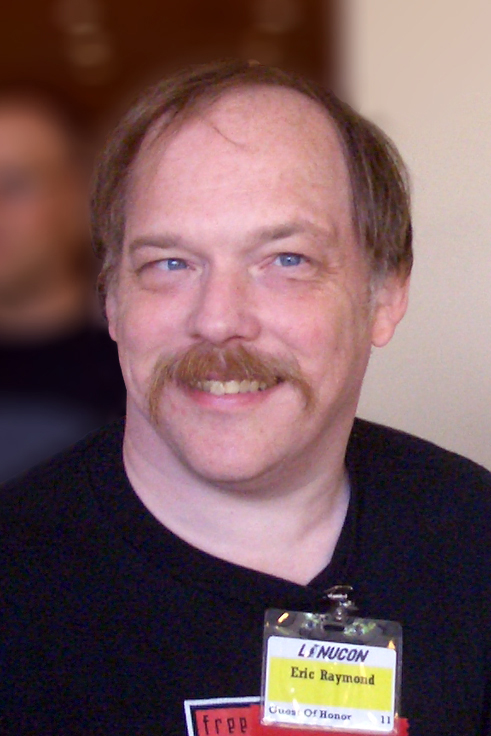
\includegraphics[width=3cm]{esr.jpg}\\
     Eric S. Raymond (1998)
   \end{center}
 \end{columns}
\end{frame}

\begin{frame}
  \frametitle{GNU/Linux}
  \begin{center}
    \begin{minipage}{0.8\textwidth}
      \begin{block}{}
        \begin{center}
          “Every good work of software starts by scratching a developer's personal itch.” - esr
        \end{center}
      \end{block}
    \end{minipage}
  \end{center}
  \begin{columns}
    \column{7cm}
      ``Hello everybody out there using minix — I’m doing a (free) operating
      system (just a hobby, won’t be big and professional like gnu)...''
    \column{3cm}
    \begin{center}
      \includegraphics[width=3cm]{linus.jpg}\\
      Linus Torvalds\\
      (1991-1992)
    \end{center}
  \end{columns}
\end{frame}

\begin{frame}
   \frametitle{\emph{Distros}}
   \begin{center}
     \renewcommand\arraystretch{2}
     \begin{tabular}{c c c}
       
\includegraphics[width=3cm]{ubuntu.png} & 
\includegraphics[width=3cm]{opensuse.png} & 
\includegraphics[width=3cm]{mint.jpg}\\
       
\includegraphics[width=3cm,trim=10mm 60mm 10mm 60mm,clip]{fedora.jpg} & 
\includegraphics[width=3cm]{debian.png} & 
\includegraphics[width=3cm]{arch.png}\\
       
\includegraphics[width=3cm]{slack.png} & 
\includegraphics[width=3cm]{redhat.jpg} & 
\includegraphics[width=3cm]{chakra.png}
     \end{tabular}
   \end{center}
\end{frame}

\begin{frame}
  \frametitle{}
  \begin{center}
    Ok, mas... E nós?
  \end{center}
\end{frame}

\begin{frame}
  \frametitle{Cultura Hacker na Educação}
  \begin{columns}
    \column{8cm}
    \begin{itemize}
    \item Ética Hacker
    \item Nelson Pretto (UFBA): ``Por uma cultura hacker na educação''
    \end{itemize}
    \column{3cm}
    
\includegraphics[width=3cm]{glider.png}
  \end{columns}
\end{frame}

\begin{frame}
   \frametitle{Open Science}
   \begin{center}
     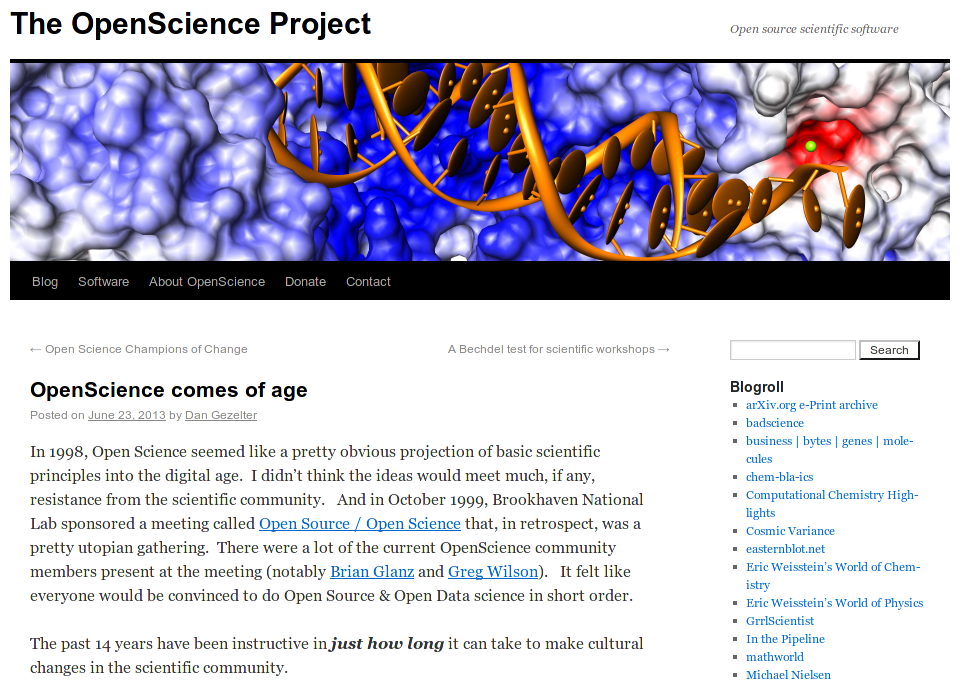
\includegraphics[width=\textwidth]{openscience.png}
   \end{center}
\end{frame}

\begin{frame}
   \frametitle{Open Access}
   \begin{columns}
     \column{7cm}
     \centering
     Acesso livre a publicações científicas
     \column{4cm}
     \begin{center}
       
\includegraphics[width=2cm]{openaccess.png}
     \end{center}
   \end{columns}
\end{frame}

\begin{frame}
  \frametitle{Formatos Abertos}
  \begin{columns}
    \column{7cm}
    \begin{itemize}
    \item Disseminação do conhecimento
    \item Garantia para o futuro
    \end{itemize}
    \column{4cm}
    \begin{center}
      
\includegraphics[width=3cm]{opendocumentformat.png}
    \end{center}
  \end{columns}
\end{frame}

\begin{frame}
   \frametitle{Softwares Matemáticos Livres}
   \begin{center}
     \begin{tabular}{l l}
       \rowcolor{purple!30} MATLAB & \uncover<2->{Octave/Scilab/Python}\\
       Photoshop & \uncover<3->{Inkscape/Gimp}\\
       \rowcolor{purple!30} Word/Excel & \uncover<4->{LibreOffice (\LaTeX !)}\\
       Geogebra & \uncover<5->{Geogebra :)}\\
       \rowcolor{purple!30} Maple & \uncover<6>{Sage}
     \end{tabular}
   \end{center}
\end{frame}

\begin{frame}
   \frametitle{Comunidade}
   Todos podem contribuir!
   \begin{itemize}
   \item Código
   \item Tradução
   \item Acessibilidade
   \item Bugs
   \item Evangelismo
   \end{itemize}
\end{frame}

\begin{frame}[fragile]
   \frametitle{Contato}
   \begin{center}
      \begin{minipage}{0.7\textwidth}
      \begin{block}{}
         \begin{center}
            \verb+@melissawm+\\
            \verb+www.mtm.ufsc.br/~melissa+
         \end{center}
      \end{block}
   \end{minipage}
   \end{center}
\end{frame}

\end{document}
